\chapter{技术路线}

\section{时空预测模型}

本系统的快反应层采用了一个基于自注意力机制的时空预测模型 \upcite {ref13_jiang2023pdformer}。这个模型由三个主要部分组成：数据嵌入层、堆叠的时空编码器层和输出层。数据嵌入层把原始输入转换成高维表示，时空编码器层用自注意力机制来建模复杂的时空依赖关系，输出层把编码结果转成最终的预测值。


\begin{figure}[H]
  \centering
  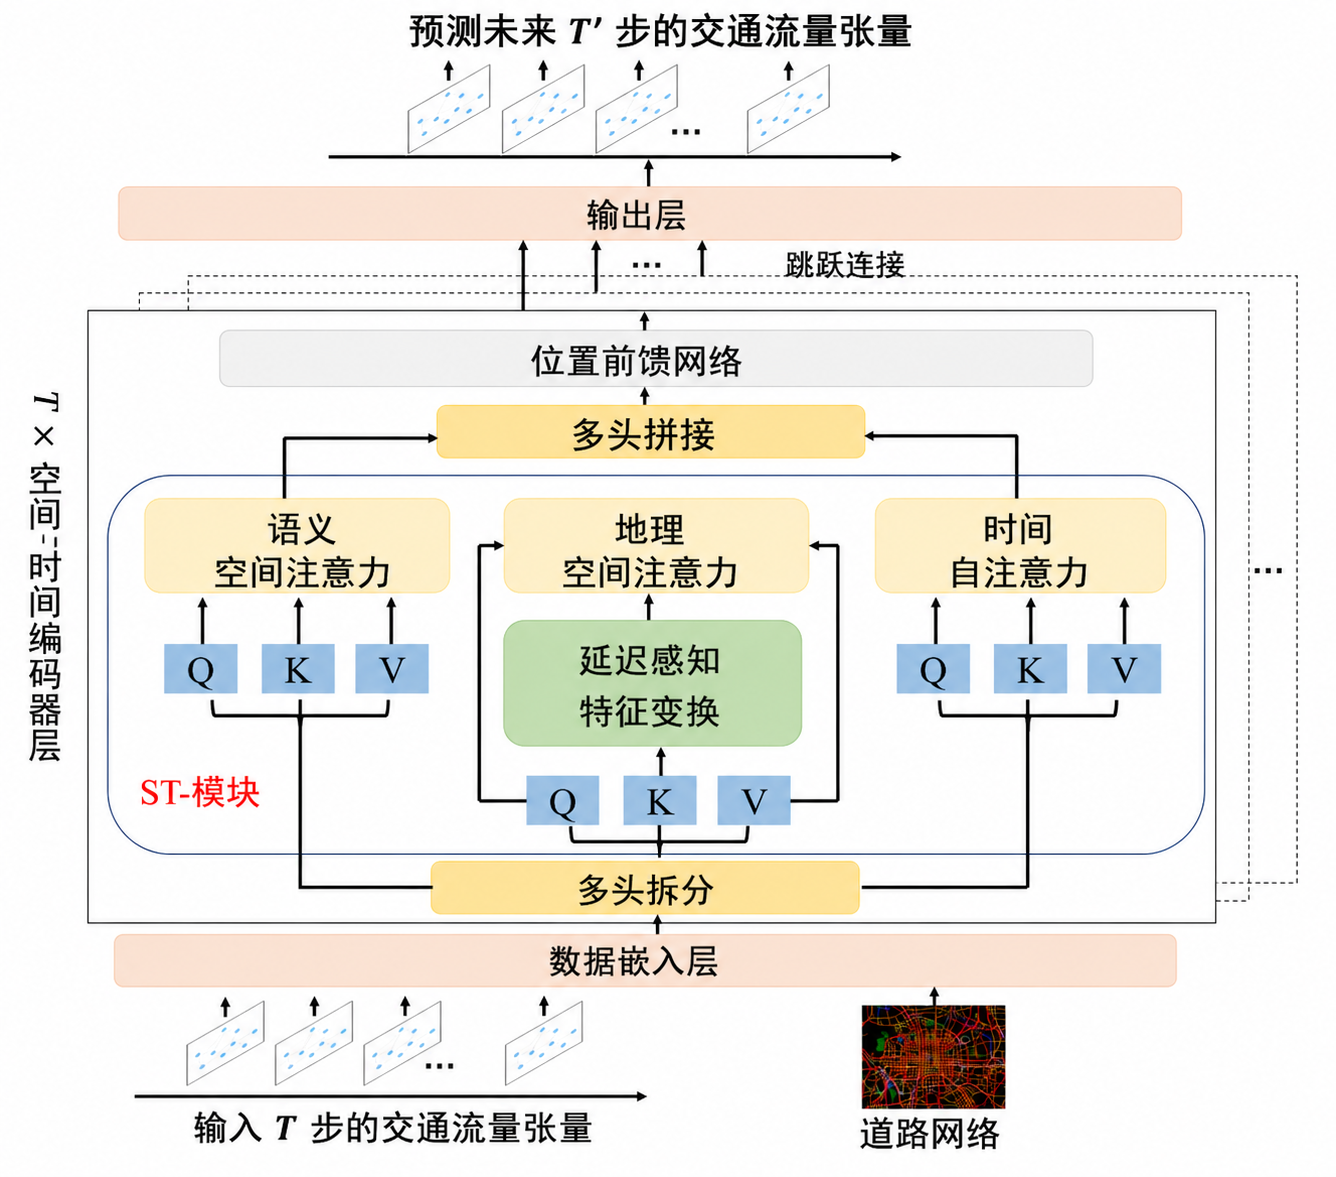
\includegraphics[width=0.9\textwidth]{figure/frame-bigcity.png}
  \caption{时空预测模型整体框架图}
  \label{fig:pdformer-framework}
\end{figure}


数据嵌入层先把原始交通数据转成模型能处理的高维特征。原始输入 $\mathcal{X} \in \mathbb{R}^{T \times N \times C}$ 通过一个全连接层映射到嵌入维度 $d$，得到 $\mathcal{X}_{data} \in \mathbb{R}^{T \times N \times d}$，其中 $T$ 是时间步数，$N$ 是路网节点数，$C$ 是输入特征的通道数。这一步的作用是把原始数值（比如车速64.375）转换到一个高维的向量空间中，让模型能够在后续的注意力计算中捕捉到更丰富的特征表示。

数据嵌入不仅要处理数值本身，还要把路网的结构信息也编进去。只用传感器编号来表示位置是不够的，因为编号是随意分配的，不包含路网中谁和谁相邻的信息。为了解决这个问题，用图拉普拉斯特征向量来编码路网的拓扑结构。先计算归一化的拉普拉斯矩阵：

为了把路网的结构信息引入模型，用图拉普拉斯特征向量来编码路网的拓扑结构。先计算归一化的拉普拉斯矩阵：

\begin{equation}
\boldsymbol{\Delta} = \boldsymbol{I} - \boldsymbol{D}^{-\frac{1}{2}} \boldsymbol{A} \boldsymbol{D}^{-\frac{1}{2}}
\end{equation}

其中 $\boldsymbol{A}$ 是邻接矩阵，$\boldsymbol{D}$ 是度矩阵，$\boldsymbol{I}$ 是单位矩阵。然后对拉普拉斯矩阵进行特征分解：

\begin{equation}
\boldsymbol{\Delta} = \boldsymbol{U}^\top \boldsymbol{\Lambda} \boldsymbol{U}
\end{equation}

取最小的 $k$ 个非平凡特征向量，通过线性投影得到空间图拉普拉斯嵌入 $\boldsymbol{X}_{spe} \in \mathbb{R}^{N \times d}$。拉普拉斯特征向量把图嵌入到了欧几里得空间中，保留了路网的全局结构信息。这样模型就能知道哪些节点在路网上是靠近的、哪些节点在结构上是连通的，而不需要手动去指定每个节点的邻居关系。

城市交通流受出行规律的影响，有很明显的周期性特征，比如早晚高峰的规律性变化。同一个路段在早上八点和凌晨两点的车流量可能差了几十倍，如果模型不知道时间信息，它就只能靠数值本身去猜，这样很难学到周期性的规律。为了解决这个问题，加入两种时间周期性嵌入，分别覆盖周周期和日周期，记为 $\boldsymbol{t}_w(t), \boldsymbol{t}_d(t) \in \mathbb{R}^d$。$w(t)$ 和 $d(t)$ 是把时间 $t$ 分别转成星期索引（1到7）和分钟索引（1到1440）的函数。把所有 $T$ 个时间步的嵌入向量拼起来，就得到了周周期嵌入 $\boldsymbol{X}_w \in \mathbb{R}^{T \times d}$ 和日周期嵌入 $\boldsymbol{X}_d \in \mathbb{R}^{T \times d}$。另外还加入了一个时间位置编码 $\boldsymbol{X}_{tpe} \in \mathbb{R}^{T \times d}$，给输入序列提供位置信息。

数据嵌入层最终的输出是上述所有嵌入向量相加的结果：

\begin{equation}
\mathcal{X}_{emb} = \mathcal{X}_{data} + \boldsymbol{X}_{spe} + \boldsymbol{X}_w + \boldsymbol{X}_d + \boldsymbol{X}_{tpe}
\end{equation}

$\mathcal{X}_{emb}$ 之后会被送入时空编码器。

时空编码器层是模型最核心的部分，基于自注意力机制来建模动态的时空依赖关系。每个编码器层包含三个关键组件：空间自注意力模块、延迟感知特征变换模块和时间自注意力模块。为了方便描述自注意力的计算过程，下面用切片符号来表示三维张量：对于 $\mathcal{X} \in \mathbb{R}^{T \times N \times D}$，$t$ 切片表示矩阵 $\boldsymbol{X}_{t::} \in \mathbb{R}^{N \times D}$，$n$ 切片表示矩阵 $\boldsymbol{X}_{:n:} \in \mathbb{R}^{T \times D}$。

空间自注意力模块用来捕捉交通数据中动态的空间依赖。在时间步 $t$，先计算查询、键和值矩阵：

\begin{equation}
\boldsymbol{Q}_t^{(S)} = \boldsymbol{X}_{t::} \boldsymbol{W}_Q^S, \quad
\boldsymbol{K}_t^{(S)} = \boldsymbol{X}_{t::} \boldsymbol{W}_K^S, \quad
\boldsymbol{V}_t^{(S)} = \boldsymbol{X}_{t::} \boldsymbol{W}_V^S
\end{equation}

其中 $\boldsymbol{W}_Q^S, \boldsymbol{W}_K^S, \boldsymbol{W}_V^S \in \mathbb{R}^{d \times d'}$ 是可学习的参数矩阵，$d'$ 是注意力计算的维度。这三句话其实是在做同一件事：把每个节点的特征表示分别映射到三个不同的空间中。查询矩阵代表“我想找什么样的邻居”，键矩阵代表“我是什么样的邻居”，值矩阵代表“我要传递什么信息”。然后在空间维度上做自注意力计算，得到所有节点之间的注意力分数：

\begin{equation}
\boldsymbol{A}_t^{(S)} = \frac{(\boldsymbol{Q}_t^{(S)})(\boldsymbol{K}_t^{(S)})^\top}{\sqrt{d'}}
\end{equation}

不同时间步的 $\boldsymbol{A}_t^{(S)} \in \mathbb{R}^{N \times N}$ 是不一样的，这就是说空间依赖关系是动态变化的。空间自注意力模块的输出为：

\begin{equation}
\text{SSA}(\boldsymbol{Q}_t^{(S)}, \boldsymbol{K}_t^{(S)}, \boldsymbol{V}_t^{(S)}) = \text{softmax}(\boldsymbol{A}_t^{(S)}) \boldsymbol{V}_t^{(S)}
\end{equation}

不过，如果让每个节点和所有其他节点都做交互，就等于把路网当成了全连接图，这样效率不高而且容易引入噪声。实际上只有部分节点对之间的交互是重要的。一种情况是距离近的节点对——相邻路段的交通状况确实会互相影响，堵车会从一条路传到旁边的路。另一种是距离远但功能相似的节点对，比如两个相隔很远的商业区可能有类似的流量变化模式，一个商业区的拥堵模式可能可以用来参考另一个商业区的流量变化。为了解决这个问题，引入了两种图掩码矩阵 $\boldsymbol{M}_{geo}$ 和 $\boldsymbol{M}_{sem}$，分别用来捕捉短距离和长距离的空间依赖。

从短距离来看，定义一个二值地理掩码矩阵 $\boldsymbol{M}_{geo}$：只有两个节点在图上的距离（跳数）小于阈值 $\lambda$ 的时候权重为1，否则为0。这样就可以把远距离节点对的注意力计算屏蔽掉，让模型只关注那些真正在路网上相邻的节点。从长距离来看，用动态时间规整（DTW）算法计算节点之间历史交通流的相似度。DTW和一般的欧几里得距离不一样的地方在于，它允许两条时间序列在时间轴上发生错位对齐，比如一条序列的峰值比另一条晚了十分钟，DTW仍然能把它们匹配上。根据DTW的相似度，为每个节点选相似度最高的 $K$ 个节点作为语义邻居，然后构建二值语义掩码矩阵 $\boldsymbol{M}_{sem}$。

基于这两种掩码矩阵，可以定义地理空间自注意力（GeoSSA）和语义空间自注意力（SemSSA）两个模块：

\begin{equation}
\text{GeoSSA}(\boldsymbol{Q}_t^{(S)}, \boldsymbol{K}_t^{(S)}, \boldsymbol{V}_t^{(S)}) = \text{softmax}(\boldsymbol{A}_t^{(S)} \odot \boldsymbol{M}_{geo}) \boldsymbol{V}_t^{(S)}
\end{equation}

\begin{equation}
\text{SemSSA}(\boldsymbol{Q}_t^{(S)}, \boldsymbol{K}_t^{(S)}, \boldsymbol{V}_t^{(S)}) = \text{softmax}(\boldsymbol{A}_t^{(S)} \odot \boldsymbol{M}_{sem}) \boldsymbol{V}_t^{(S)}
\end{equation}

其中 $\odot$ 表示逐元素相乘。这样空间自注意力模块就同时考虑了短距离的地理邻域和长距离的语义邻域。

实际交通中有一个很重要的现象：拥堵不会瞬间传遍整个路网，而是需要时间的。比如一个路段出了事故，可能要过几分钟才会影响到旁边的路段。如果模型不把这个延迟考虑进去，它可能会以为所有路段之间的影响是同步发生的，这显然不符合真实情况 \upcite{ref66_wang2025congestion}。延迟感知特征变换模块就是为了建模这种传播延迟，它把延迟信息引入到地理空间自注意力的键矩阵里面。

具体做法是这样的。先从历史交通数据里提取一组有代表性的短期交通模式。用大小为 $S$ 的滑动窗口把历史数据切成一段段的交通流序列，然后用 k-Shape 聚类算法对这些序列做聚类。k-Shape 是一种专门针对时间序列的聚类方法，它跟普通的聚类算法不一样的地方在于，它关注的是序列的形态而不是绝对值的大小。比如一条从30到60的上升趋势和一条从80到110的上升趋势在k-Shape看来是相似的，因为它们的“形状”是一样的。每个聚类中心 $\boldsymbol{p}_i$ 代表一种交通模式，长度也是 $S$。聚类结果集合记为 $\mathcal{P} = \{\boldsymbol{p}_i | i \in [1, \cdots, N_p]\}$，$N_p$ 是聚类总数。

对于节点 $n$ 从时间步 $(t - S + 1)$ 到 $t$ 的历史交通流序列 $\boldsymbol{x}_{(t-S+1:t), n}$，先用嵌入矩阵 $\boldsymbol{W}_u$ 得到高维表示：

\begin{equation}
\boldsymbol{u}_{t,n} = \boldsymbol{x}_{(t-S+1:t), n} \boldsymbol{W}_u
\end{equation}

再用另一个嵌入矩阵 $\boldsymbol{W}_m$ 把每个交通模式序列转成记忆向量：

\begin{equation}
\boldsymbol{m}_i = \boldsymbol{p}_i \boldsymbol{W}_m
\end{equation}

然后计算历史交通流表示和交通模式记忆向量之间的相似度：

\begin{equation}
w_i = \text{softmax}(\boldsymbol{u}_{t,n}^\top \boldsymbol{m}_i)
\end{equation}

根据这个相似度对交通模式集做加权求和，就得到了集成历史序列表示：

\begin{equation}
\boldsymbol{r}_{t,n} = \sum_{i=1}^{N_p} w_i (\boldsymbol{p}_i \boldsymbol{W}_c)
\end{equation}

其中 $\boldsymbol{W}_c$ 是可学习的参数矩阵。$\boldsymbol{r}_{t,n}$ 包含了节点 $n$ 在时间窗口内的历史交通流信息。最后，用 $N$ 个节点的集成表示 $\boldsymbol{R}_t$ 来更新键矩阵：

\begin{equation}
\tilde{\boldsymbol{K}}_t^{(S)} = \boldsymbol{K}_t^{(S)} + \boldsymbol{R}_t
\end{equation}

其中 $\boldsymbol{R}_t \in \mathbb{R}^{N \times d'}$ 由 $N$ 个节点的所有集成表示拼接而成。这样新的键矩阵 $\tilde{\boldsymbol{K}}_t^{(S)}$ 就包含了所有节点近期的历史交通信息，当计算查询矩阵和新的键矩阵的乘积时，查询就可以感知到其他节点的历史交通状况，实现了对传播时间延迟的显式建模。

交通流在不同时间步之间也有依赖关系，比如周期性变化或者某种趋势，而且这些依赖关系在一天中不同的时段是不一样的。举个例子，早高峰期间，车流量变化很快，近期的几个时间步对预测的帮助很大；但在深夜时段，路况比较稳定，更早的时间步可能也有参考价值。时间自注意力模块就是用来发现这些动态的时间模式的。对于节点 $n$，先计算查询、键和值矩阵：

\begin{equation}
\boldsymbol{Q}_n^{(T)} = \boldsymbol{X}_{:n:} \boldsymbol{W}_Q^T, \quad
\boldsymbol{K}_n^{(T)} = \boldsymbol{X}_{:n:} \boldsymbol{W}_K^T, \quad
\boldsymbol{V}_n^{(T)} = \boldsymbol{X}_{:n:} \boldsymbol{W}_V^T
\end{equation}

其中 $\boldsymbol{W}_Q^T, \boldsymbol{W}_K^T, \boldsymbol{W}_V^T \in \mathbb{R}^{d \times d'}$ 是可学习的参数。然后在时间维度上做自注意力计算，得到节点 $n$ 在所有时间步之间的依赖关系：

\begin{equation}
\boldsymbol{A}_n^{(T)} = \frac{(\boldsymbol{Q}_n^{(T)})(\boldsymbol{K}_n^{(T)})^\top}{\sqrt{d'}}
\end{equation}

这里的 $\boldsymbol{A}_n^{(T)} \in \mathbb{R}^{T \times T}$ 是一个注意力权重矩阵，矩阵中第 $i$ 行第 $j$ 列的值表示节点 $n$ 在时间步 $i$ 的状态对时间步 $j$ 的影响有多大。和空间自注意力一样，这个权重也是通过数据学习得到的，不同节点之间的时间依赖模式可以不一样。同时由于它对所有时间步之间都做两两计算，所以即使相隔很远的时间步也能直接产生依赖，解决了RNN中存在的信息衰减问题。

时间自注意力可以捕捉不同节点各自不同的动态时间模式，而且由于它能看到所有时间步，可以建模长距离的时间依赖。时间自注意力的输出为：

\begin{equation}
\text{TSA}(\boldsymbol{Q}_n^{(T)}, \boldsymbol{K}_n^{(T)}, \boldsymbol{V}_n^{(T)}) = \text{softmax}(\boldsymbol{A}_n^{(T)}) \boldsymbol{V}_n^{(T)}
\end{equation}

上面介绍了三种注意力机制，它们分别从地理空间、语义空间和时间三个维度捕捉了交通数据中的依赖关系。但空间和时间的信息不是独立的——交通状况在空间上的传播会随着时间变化，时间上的周期性也受到路网结构的约束。所以不能把空间和时间的信息分开处理完再简单拼起来，而是需要把它们融合到一个统一的计算框架中。具体做法是，把这些注意力机制融合到一个多头自注意力块中。注意力头包括三种类型：地理头（GeoSAH）、语义头（SemSAH）和时间头（TAH），分别对应上面说的三种注意力机制。把这些头的输出拼接起来再做一个线性投影，就得到了最终的输出。这样模型可以同时整合空间和时间的信息。时空自注意力块的公式如下：

\begin{equation}
\text{STAttn} = \bigoplus(\mathcal{Z}_{1\cdots h_{geo}}^{geo}, \mathcal{Z}_{1\cdots h_{sem}}^{sem}, \mathcal{Z}_{1\cdots h_{t}}^{t}) \boldsymbol{W}_O
\end{equation}

$\bigoplus$ 表示拼接操作，$\mathcal{Z}^{geo}, \mathcal{Z}^{sem}, \mathcal{Z}^{t}$ 分别是地理头、语义头和时间头的输出拼接，$h_{geo}, h_{sem}, h_t$ 是三种注意力头的数量，$\boldsymbol{W}_O \in \mathbb{R}^{d \times d}$ 是可学习的投影矩阵。维度设置是 $d' = d / (h_{geo} + h_{sem} + h_t)$。

在多头自注意力的输出上还会接一个逐位置的全连接前馈网络，加上层归一化和残差连接，得到时空编码器层的输出 $\mathcal{X}_o \in \mathbb{R}^{T \times N \times d}$。

最后是输出层。在每个时空编码器层之后，用 $1 \times 1$ 卷积做跳跃连接，把输出转到跳跃维度 $\mathcal{X}_{sk} \in \mathbb{R}^{T \times N \times d_{sk}}$，$d_{sk}$ 是跳跃维度。然后把所有跳跃连接层的输出加起来，得到最终的隐藏状态 $\mathcal{X}_{hid} \in \mathbb{R}^{T \times N \times d_{sk}}$。要做多步预测的话，用输出层把隐藏状态转成目标维度：

\begin{equation}
\hat{\mathcal{X}} = \text{Conv}_2(\text{Conv}_1(\mathcal{X}_{hid}))
\end{equation}

其中 $\hat{\mathcal{X}} \in \mathbb{R}^{T' \times N \times C}$ 是 $T'$ 步的预测结果，$\text{Conv}_1$ 和 $\text{Conv}_2$ 都是 $1 \times 1$ 卷积。这里选择直接多步预测而不是递归预测，因为直接预测可以避免累积误差，而且效率更高。

以上就是时空预测模型的全貌。回顾整个模型的设计，每一层的选择都和交通数据的具体特点对应。交通数据是多维的，所以数据嵌入层用全连接做维度映射 \upcite{ref14_yin2026dgctransformer}。交通数据有路网结构，所以用图拉普拉斯嵌入把拓扑信息编进去。交通数据有周期规律，所以用周嵌入和日嵌入把时间周期信息告诉模型。交通数据的空间依赖是动态变化的——相邻路段的影响程度不是固定的，而是随着交通状况变化的，所以用自注意力替代固定邻接矩阵来建模空间关系。路网中远距离的节点之间也可能有相似的变化模式，所以用语义掩码加DTW来捕捉长距离的语义邻居。拥堵在路网中的传播不是瞬时的而是有延迟的，所以用延迟感知特征变换模块把历史流量模式整合到注意力计算中。交通流在时间维度上也有复杂的依赖关系，不同时间步之间的影响在不同节点上是不一样的，所以用时间自注意力来建模动态的时间模式。最后，空间和时间的注意力结果不是独立处理的，而是通过异质注意力融合到一个统一的多头框架中，让空间和时间的信息在同一个计算过程中互相影响。这种从数据特点出发逐层设计的方式，让模型能够从海量交通数据中提取出有价值的时空模式，为智能体的分析决策提供准确的预测支持。

\section{原子文件与MCP时空上下文}

交通数据来自各种不同类型的采集设备，有固定在道路上的传感器、有出租车和网约车的GPS轨迹、还有收费站的ETC记录。这些数据在格式、采样频率和表示方式上差异很大，如果直接把它们扔给预测模型或者智能体来处理显然是不行的。所以在本项目中，第一步需要做的，是把各种异构的交通数据统一成一个标准化的格式。这个标准化格式就是ST原子文件（Spatio-Temporal Atomic Files），也就是时空原子文件 \upcite{ref63_JSJYGG202118006}。

原子文件的设计需要先想清楚交通数据的本质是什么。交通数据本质上是一种时空数据，它描述的是“什么东西在什么时间什么位置发生了什么变化”。其中“什么东西”指的是具体的数据采集对象——一个传感器节点或者一条路段；“什么位置”是这个对象在路网中的空间坐标；“什么时间”是数据记录的时刻；“发生了什么变化”则是该对象在那一时刻的交通状态值，比如流量或交通占有率。这四个要素合在一起，才能完整地描述一条交通数据记录的意义。如果缺少其中一个，数据就是残缺的——只知道车速不知道位置，或者只知道位置不知道时间，都没有实际用处。仔细拆解一下，这四个要素又可以归并为三个基本要素：空间实体（什么东西在什么位置）、实体之间的关系（各个实体在路网中如何连接）、以及动态状态（实体在不同时间发生了什么变化）。接下来是对这三个基本要素的介绍。

第一个要素是空间实体。任何交通数据都对应的某个物理对象——一个传感器、一条路段、一个交叉口、或者一个区域网格。每个实体都有自己的位置信息，比如经纬度坐标；有自己的几何类型，是点状、线状还是面状；还有自己的固有属性，比如传感器的编号、路段的长度、车道的数量。这些信息在时间上是相对稳定的。在本项目中，处理的主要是点状的数据，空间实体的属性是点状的。所以空间实体描述的是交通系统中“谁在哪里”这个静态问题。

第二个要素是实体之间的关系。交通实体不是散落在地图上的孤立点，它们之间通过路网相互连接。这种连接关系构成了路网的拓扑结构。如果有一堆传感器，只知道每个传感器的位置是不够的，还需要知道哪些传感器是相邻的、从A传感器到B传感器经过哪些中间节点、两个传感器之间的距离是多远。如果不记录这些关系，模型就不知道路网是长什么样的，也就没有办法理解拥堵是如何在路网上传播的。所以实体关系描述的是“谁和谁相连”这个结构性静态问题，需要解决如何构建路网的问题。

第三个要素是动态状态。这是交通数据最有价值的部分。同一个路段在早高峰和午夜的状态可能差了几十倍，而且这些变化不是随机的，而是有规律的——每天有早晚高峰的周期性、每周有工作日和周末的差异、还可能受到交通事故和天气等突发因素的影响。如果不记录这些随时间变化的数据，那就只剩下地图上的一些静止的点，做不了任何预测。所以动态状态描述的是“实体发生了什么变化”这个问题。

基于上面这三个维度的分析，就得到了一种自然的数据组织方式：用 \texttt{.geo} 文件来存储空间实体的信息，回答“谁在哪里”；用 \texttt{.rel} 文件来存储实体之间的关系信息，回答“谁和谁相连”；用 \texttt{.dyna} 文件来存储动态状态信息，回答“发生了什么变化”。这三种文件类似于csv文件,即含有多列数据的表格文件，每行记录一个实体、一个关系或者一个状态变化事件。每个文件都包含了一个主键列来唯一标识每条记录，还有一些属性列来描述记录的具体内容。

这三种文件合在一起，就是一套完整的ST原子文件格式。不论原始数据来自哪个城市、哪个传感器网络，只要按照这种格式来组织数据，上层的预测模型和智能体面对的就是统一的数据接口，不需要关心底层的数据源差异。这也对应了BigCity时空大模型的强泛化性能力。下表列出了这几种原子文件的具体格式。对于不同的交通预测任务，同一个数据集不一定包含全部类型的原子文件，本系统主要使用了 .geo、.rel、.dyna 和 config.json 四种。


\begin{table}[H]
\centering
\caption{原子文件格式定义}
\label{tab:atomic-files}
\begin{tabular}{p{2.5cm}|p{4cm}|p{6cm}}
\hline
文件名 & 内容 & 示例 \\
\hline
\tt .geo & 地理实体属性信息，包括实体ID、类型和坐标位置 & \tt geo\_id, type, coordinates \\
\hline
\tt .rel & 实体间的关系信息，描述路网的拓扑连接结构 & \tt rel\_id, type, origin\_id, destination\_id \\
\hline
\tt .dyna & 交通状态动态变化信息，记录每个实体在不同时间步的状态 & \tt dyna\_id, type, time, entity\_id, properties \\
\hline
\tt config.json & 描述各表的数据类型、字段含义和数据集参数 & \tt geo.types, info.data\_col, output\_dim \\
\hline
\end{tabular}
\end{table}

\texttt{.geo} 文件对应的是空间实体这个要素。在交通场景中，实体可以是一个传感器节点、一个路段、一个交叉口或者一个区域网格。每条记录包含四个部分。第一是 \texttt{geo\_id}，主键，唯一确定一个地理实体，相当于每个实体在系统中的身份证号。第二是 \texttt{type}，表示实体的几何类型，有点（Point）、线（LineString）和面（Polygon）三种取值，与 GeoJSON 标准中的点线面一致。第三是 \texttt{coordinates}，由 float 类型组成的数组或嵌套数组，描述实体的位置信息。对于传感器和路口这种点状实体，坐标就是一个经纬度对，比如 \texttt{[116.35, 39.95]}。对于路段这种线状实体，坐标就是一系列经纬度点组成的线段，比如 \texttt{[[116.35,39.95],[116.36,39.96]]}。对于区域这种面状实体，坐标就是由多个顶点围成的多边形。第四是 \texttt{properties}，描述实体的属性信息，可以有多个列。比如对于网格数据，必须包含 \texttt{row\_id} 和 \texttt{column\_id} 两列来表示网格的行列编号。对于传感器节点，属性列可以是传感器的名称或功能类型。

\texttt{.rel} 文件对应的是实体关系这个要素。如果说 \texttt{.geo} 文件告诉系统有哪些节点，那么 \texttt{.rel} 文件告诉系统这些节点是怎么连在一起的。每条记录包含五个部分。\texttt{rel\_id} 是主键，唯一确定一条关系。\texttt{type} 表示关系类型，取值可以是 \texttt{geo}（基于地理实体的关系）或 \texttt{usr}（基于用户的关系），在路网场景中通常使用 \texttt{geo} 类型。\texttt{origin\_id} 是关系起点方的ID，\texttt{destination\_id} 是终点方的ID。举个例子，如果传感器101和传感器102在路网上是相邻的，那么 \texttt{.rel} 文件中就会有一条记录 \texttt{(0, geo, 101, 102)} 来表示这个连接。\texttt{properties} 是关系的属性列，最重要的就是权重列，通常表示两个传感器之间的路段长度或者平均通行时间。这些权重在构建邻接矩阵的时候非常关键——邻接矩阵告诉模型路网的结构，有了它模型才能在空间维度上做图卷积或者注意力计算。在 config.json 中，需要通过 \texttt{weight\_col} 字段指定从 .rel 文件中加载哪一列作为权重，并通过 \texttt{set\_weight\_link\_or\_dist} 字段控制是使用权重原始值还是将其二值化。

\texttt{.dyna} 文件对应的是动态状态这个要素，也是原子文件中数据量最大、最核心的一个。它记录了交通系统中各个实体在不同时间步上的状态变化。每条记录包含 \texttt{dyna\_id}（记录的唯一ID）、\texttt{type}（数据类型，如 \texttt{state} 表示状态数据、\texttt{trajectory} 表示轨迹数据）、\texttt{time}（时间戳，采用ISO-8601标准格式，如 \texttt{2012-03-01T00:00:00Z}）、\texttt{entity\_id}（关联的实体ID，指向 \texttt{.geo} 文件中的某个传感器或路段）以及 \texttt{properties}（具体的属性值，可以有多个列，比如既有速度数据又有流量数据）。对于交通状态预测任务，\texttt{entity\_id} 通常是传感器的编号，每条记录表示某个传感器在某个时间点的观测值。而对于网格结构的数据，\texttt{entity\_id} 会变成两列 \texttt{row\_id} 和 \texttt{column\_id}，文件后缀也变为 \texttt{.grid}。对于基于OD结构的数据，\texttt{entity\_id} 变为 \texttt{origin\_id} 和 \texttt{destination\_id}，后缀为 \texttt{.od}。\texttt{.dyna} 文件的数据按照实体ID和时间双关键字排序——同一个实体的记录放在一起并按时间从早到晚排列，这样模型读取时可以直接按顺序处理。比如一条传感器数据 \texttt{(0, state, 2012-03-01T00:00:00Z, 773869, 64.375)}，表示2012年3月1日零点传感器773869的车速是64.375，紧接着下一条就是同一传感器在五分钟后的数据。

有了 \texttt{.geo}、\texttt{.rel} 和 \texttt{.dyna} 三种原子文件，就可以把交通数据集统一成标准化的表示。但光有数据还不够，还需要一个文件来描述这些数据的具体含义和配置参数，这就是 \texttt{config.json} 的作用。config.json 以 JSON 格式保存，包含 \texttt{geo}、\texttt{rel}、\texttt{dyna}、\texttt{ext} 和 \texttt{info} 等键。\texttt{geo} 和 \texttt{dyna} 键中通过 \texttt{including\_types} 数组声明文件中有哪些 type，然后为每个 type 说明对应的 properties 列名和数据类型——比如 \texttt{geo\_id} 是离散ID、\texttt{traffic\_speed} 是数值、\texttt{poi\_name} 是字符串。\texttt{info} 键中包含了数据集的运行参数，比如 \texttt{data\_col} 指定从数据文件中加载哪些列作为特征、\texttt{output\_dim} 指定模型输出的维度、\texttt{time\_intervals} 说明数据的时间片长度（以秒为单位）、\texttt{weight\_col} 指定从 .rel 文件中加载权重列、\texttt{calculate\_weight\_adj} 决定是否对邻接矩阵应用高斯核变换。有了 config.json，系统就知道数据文件中有哪些字段、每个字段是什么类型、模型需要哪些输入输出参数，从而可以自动完成数据加载和预处理，不需要为每个数据集单独写代码。

下图用ER图的形式展示了一个典型的原子文件结构示例。图中用矩形表示实体表（Geo、Rel、Dyna），用菱形表示实体之间的业务联系，用椭圆表示每个表的属性字段。Geo 表是核心实体，它记录了交通网络中每个空间节点的基本信息——geo\_id 作为唯一标识，type 字段区分节点的几何类型（点、线或面），coordinates 字段存储经纬度坐标或坐标序列，properties 字段存放传感器名称、功能类型等附加属性。每个 Geo 实体通过“作为起点”和“作为终点”两种关系与 Rel 表相连，这意味着一条 Rel 记录总是连接两个 Geo 实体，一个 Geo 实体可以同时出现在多条 Rel 记录的起点和终点位置。Rel 表本身记录了节点之间的连接关系和权重（cost），这个权重在实际数据中对应路段长度或平均通行时间，是构建路网邻接矩阵的关键参数。同时 Geo 表通过“拥有状态”关系与 Dyna 表相连，这是一个一对多的关系——一个 Geo 实体对应多条 Dyna 记录，每条记录对应一个时间步的状态。Dyna 表记录了每个 Geo 实体在不同时间步上的动态状态数据，属性字段包括时间戳 time、实体编号 entity\_id，以及交通流量 traffic\_flow、平均车速 speed、道路占有率 occupancy 等数值指标。

\begin{figure}[H]
  \centering
  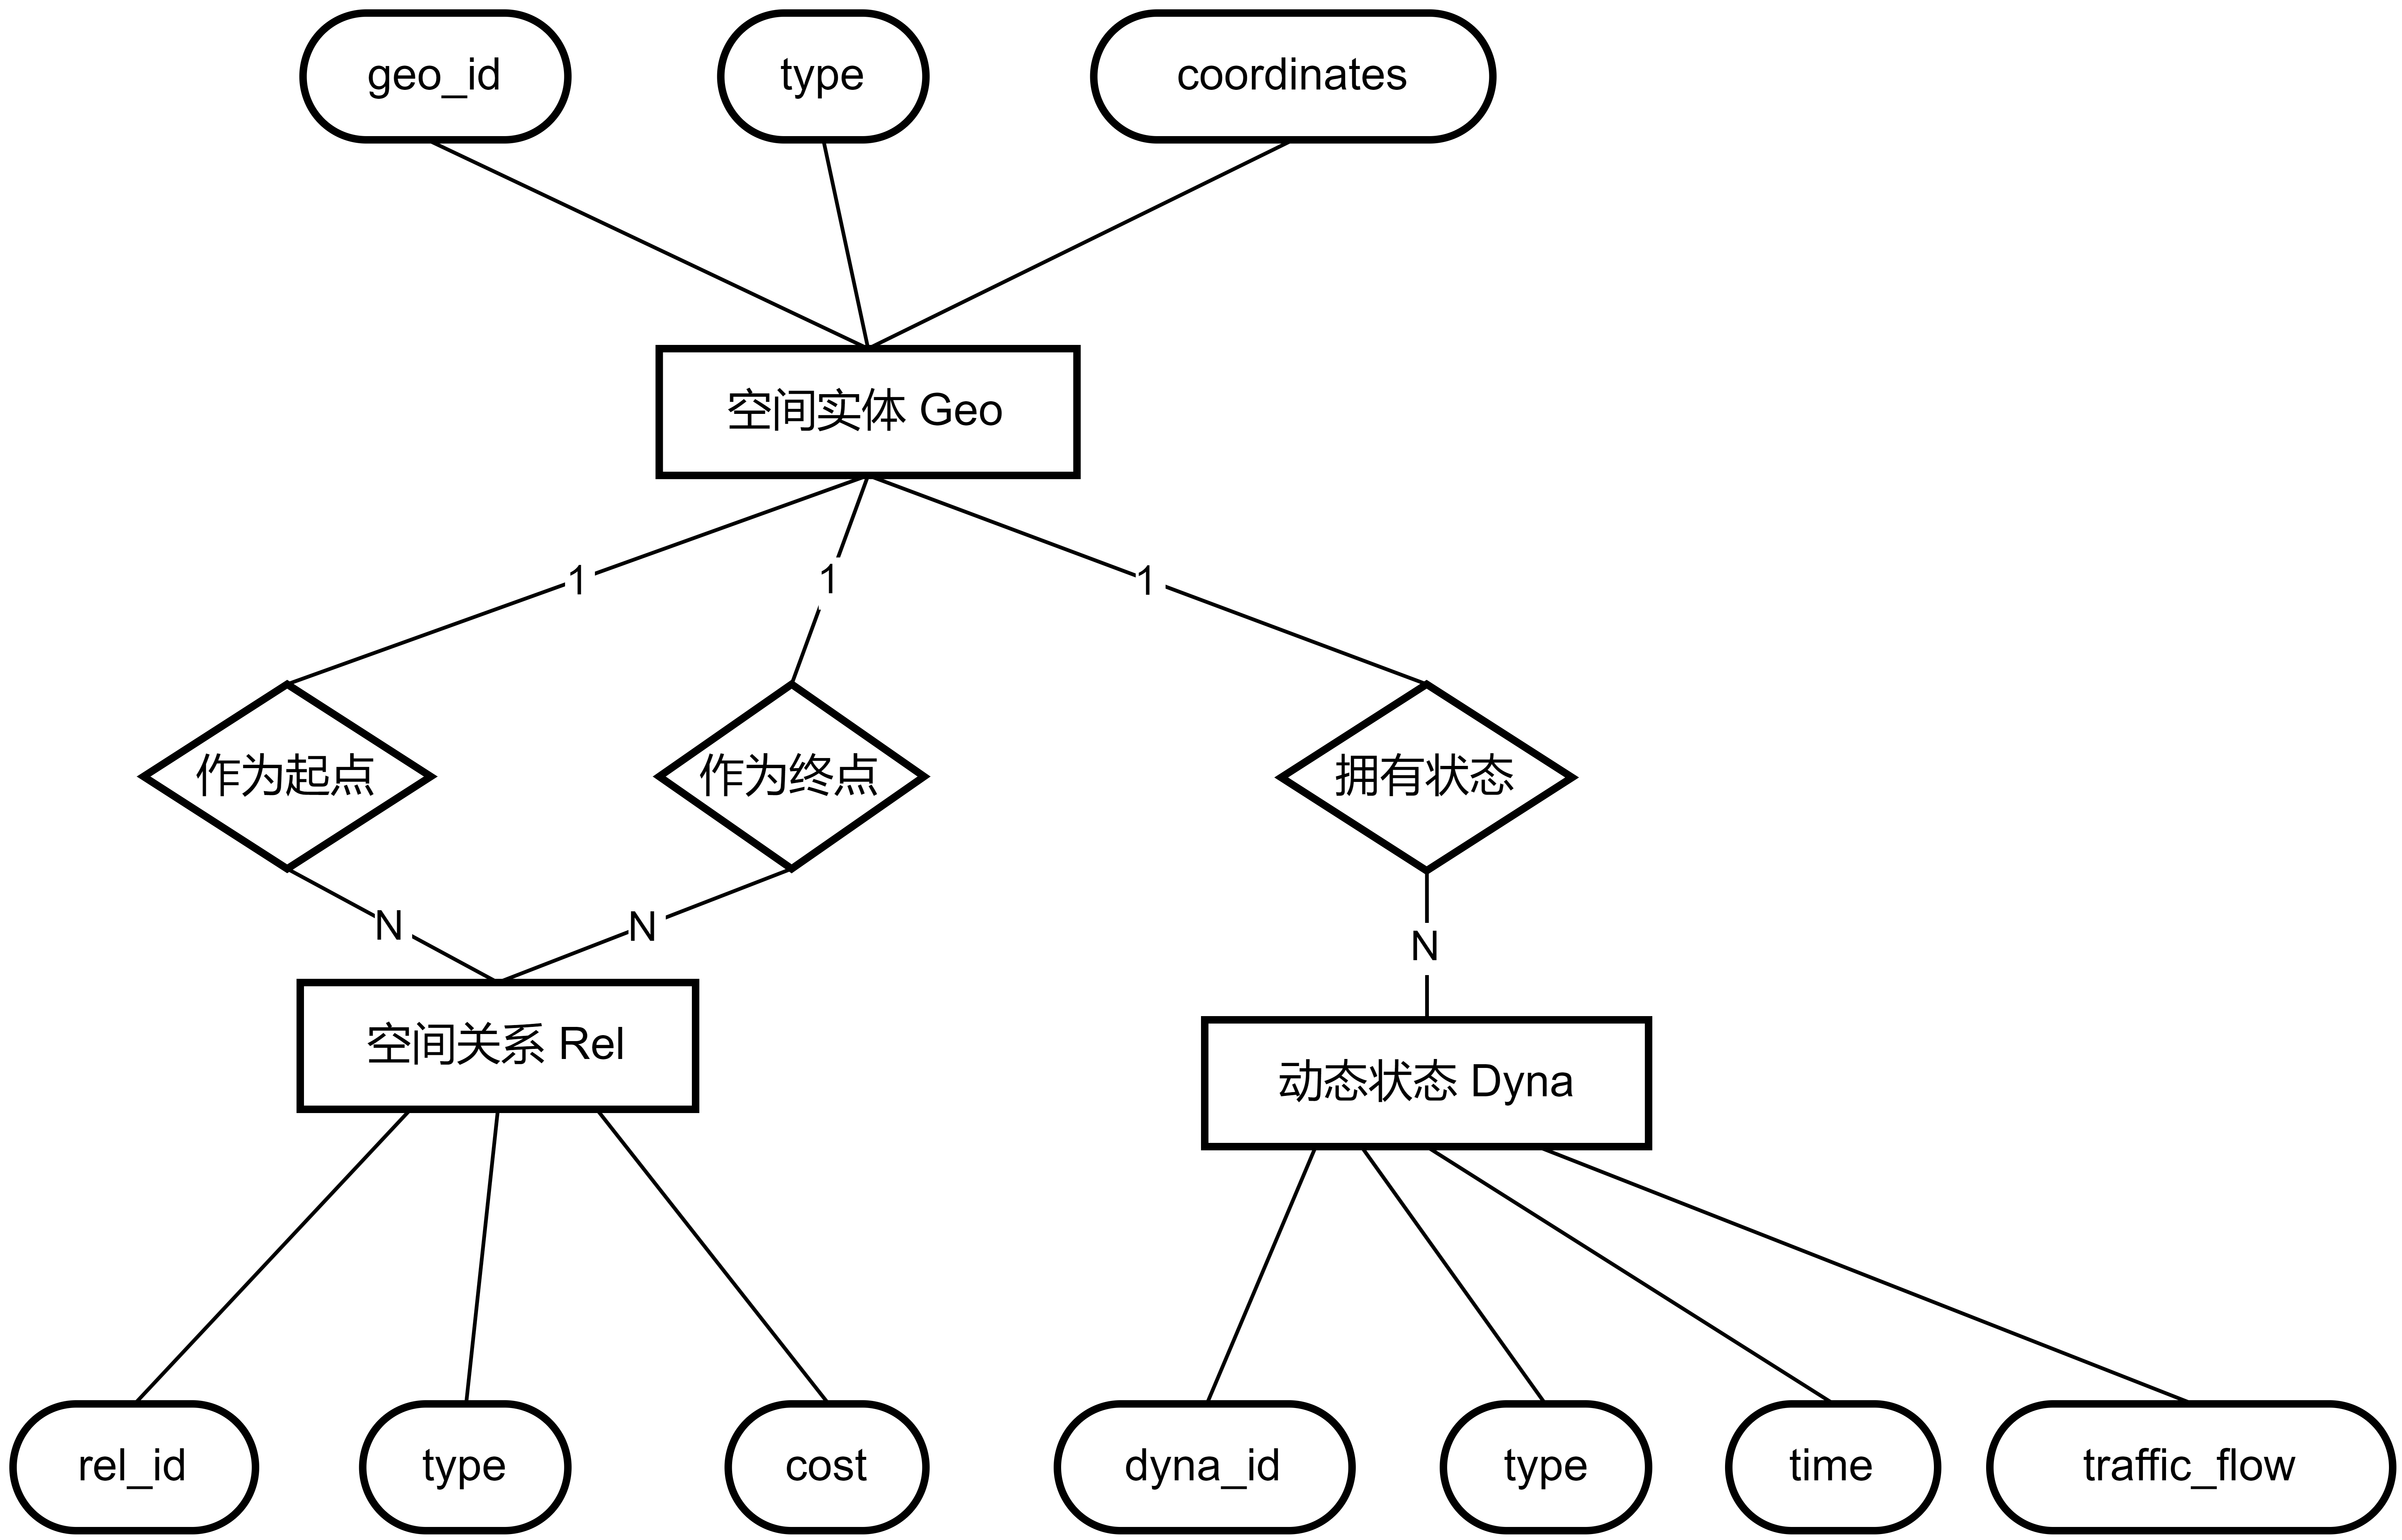
\includegraphics[width=0.65\textwidth]{figure/ER图.drawio.png}
  \caption{原子文件结构ER图示例}
  \label{fig:er-diagram}
\end{figure}

用一个具体的例子来说明这三张表是如何协同工作的。以 PeMS08 数据集为例，模型要预测未来一小时传感器101的交通流量，它的输入需要三方面的信息。首先从 Geo 表中读取传感器101的经纬度坐标和几何类型，确定它的空间位置。然后从 Rel 表中找出与传感器101相邻的所有传感器节点以及它们之间的距离（cost），这些信息构成了路网的拓扑结构，是模型进行空间聚合的基础。最后从 Dyna 表中提取传感器101及其相邻节点在过去一小时内的历史流量序列——每五分钟一个数据点，共十二个时间步。这三部分数据组装在一起，就形成了模型一次推理所需的完整输入：空间位置告诉模型“数据来自哪里”，拓扑关系告诉模型“路网结构是什么样的”，历史序列告诉模型“过去一小时交通状况如何变化”。三张表联合起来，才能给模型提供完整的时空上下文。


原子文件解决了数据统一表示的问题，但智能体系统还需要知道这些数据能怎么用、通过什么方式来获取。这就引出了MCP。MCP（Model Context Protocol）在这里扮演的角色，是把原子文件封装成智能体可以直接调用的标准化工具接口。MCP规定了每个工具的描述方式、输入参数格式和返回值格式，大语言模型不需要理解底层的数据存储细节，只需要按照协议规范发出调用请求，就能获取到需要的数据。

具体来说，\texttt{.geo} 文件对应了空间上下文相关的工具——智能体可以调用这些工具查询某个路段的位置信息、获取相邻路段列表或者检索某个区域内的所有传感器节点。\texttt{.rel} 文件对应了拓扑上下文相关的工具——智能体可以调用这些工具获取两个节点之间的最短路径、计算路网的邻接矩阵或者判断两个节点是否连通。\texttt{.dyna} 文件对应了动态上下文相关的工具——智能体可以调用这些工具查询某个路段在某个时间段的历史流量序列，或者调用预测模型获取未来一段时间内的流量预测。MCP把这三类工具统一到一个协议框架下，每个工具都有明确的接口定义，智能体只需要知道工具的名字和它能做什么，不需要关心后台是从数据库读数据还是从模型算结果。

通过原子文件和MCP的分层设计，系统实现了交通数据表示和智能体工具调用的解耦。原子文件把异构数据变成了统一格式，解决了“数据怎么存”的问题。MCP把这些统一格式的数据封装成了服务接口，解决了“数据怎么用”的问题。这样在实际部署的时候，即使换了新的数据源或者改了底层的存储方式，只要原子文件的格式和MCP的接口规范不变，上层的智能体和预测模型就不需要做任何修改。这种设计正是系统可扩展性和灵活性的基础。

\section{基于ReAct与LangGraph的智能体流程}

上面介绍了预测模型和数据处理的具体技术，但还有一个关键问题：慢思考层的大语言模型是怎么和快反应层的工具协同工作的？这个过程由基于ReAct范式的智能体流程来控制。ReAct是"Reasoning + Acting"的缩写，也就是“推理加行动”，最早来自Yao等人在2023年提出的框架 \upcite{ref36_yao2023react}。它的核心思路是让大语言模型在一个循环里交替进行推理和行动：先根据当前的任务目标推理出下一步需要做什么，然后调用工具获取信息或执行操作，拿到结果后再进入下一轮推理。这样一步步走下去直到任务完成，而不是一次性把所有步骤都想好再动手。选择ReAct而非其他方法，是因为交通分析任务本身就需要这种迭代的方式——比如用户问“学院路今天早高峰比上周同期堵了多少”，智能体需要先去查今天的数据，然后去查上周同期的数据，对比之后才能回答。链式思维（Chain-of-Thought）只能凭空推理无法获取实时数据，单纯的工具调用又缺少推理的灵活性，ReAct正好在两者之间找到了平衡。

ReAct循环在代码层面通过LangGraph框架来实现。LangGraph是LangChain团队推出的一个用于构建有状态多步工作流的框架，与一般的链式调用不同，它把工作流组织成一个有向状态图（StateGraph）。图中的每个节点执行一个具体的操作，节点之间的边定义了执行顺序和条件判断逻辑。基于这种图架构，可以根据中间结果动态决定下一步走哪条路，而不是提前把每一步都写死。系统的智能体架构就是在LangGraph的状态图上搭建的，整条流程从用户输入开始，经过用户输入、意图理解、工具调用、结果分析几个阶段，最后输出分析报告，如下图所示。


\begin{figure}[H]
  \centering
  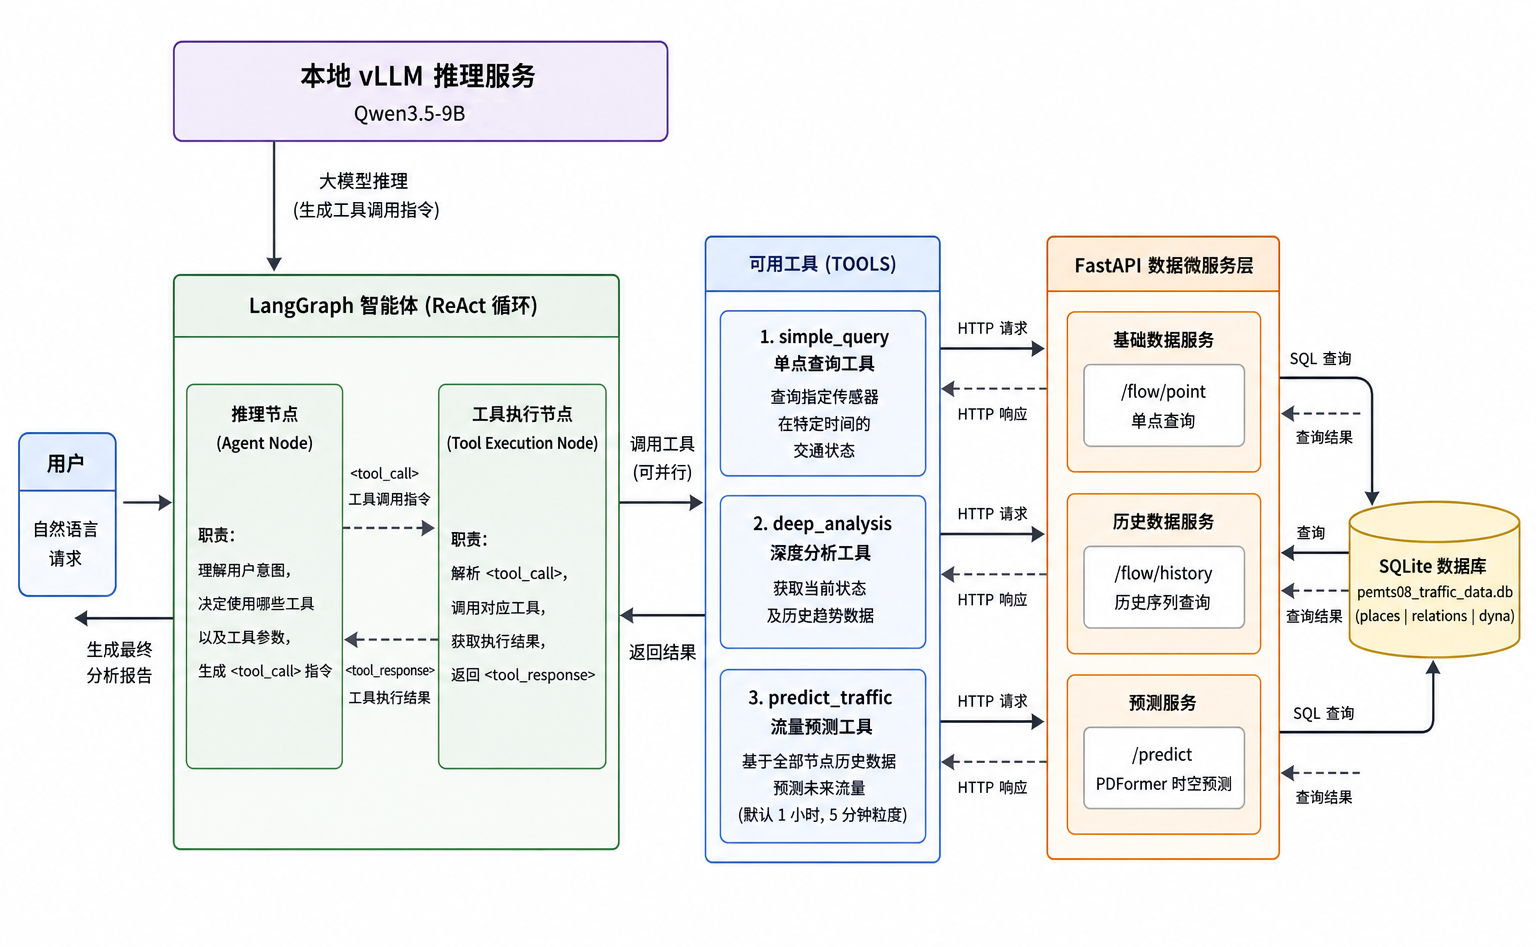
\includegraphics[width=0.9\textwidth]{figure/image14.png}
  \caption{智能体架构设计}
  \label{fig:agent-architecture}
\end{figure}

流程大致包含五个步骤。第一步是用户输入，用户用自然语言提出交通分析需求，比如“查一下北三环当前的车速”或者“预测一下明天早高峰学院路的拥堵情况”，用户的指令作为初始状态传入状态图。第二步是意图理解与任务分解，状态图进入推理节点，大语言模型根据系统提示词中的工具列表来理解用户需求，把模糊的自然语言指令拆解成具体的子任务——比如“对比北三环和西二环今天的拥堵情况”，模型会识别出需要分别查询两个路段的数据然后对比分析。第三步是工具调度与执行，如果大模型判断需要调用工具，状态图通过条件路由边进入工具执行节点，接收模型发出的指令去调用后端服务，这一步可以并行调用多个不互相依赖的工具来减少等待时间。第四步是结果分析与循环判断，推理节点收到执行结果后检查信息是否足够，不够则继续生成下一轮工具调用、状态图再次进入工具执行节点，够了则直接生成最终报告、状态图结束循环。第五步是输出结果，最终的分析报告以自然语言文本的形式返回给用户，其中包含智能体的分析过程和得出结论的依据。

下图用时序图展示了上述五个步骤中各个模块之间的消息传递顺序和时间关系。整个流程分为三个阶段。第一阶段是用户到系统，用户发送自然语言指令后推理节点进行意图理解和任务分解。第二阶段是循环执行，推理节点下发工具调用指令（可以并行下发多个），工具执行节点调用后端服务获取数据后返回结构化结果，推理节点对结果进行分析并判断是否需要继续循环。第三阶段是输出结果，推理节点在确认信息足够后生成最终的分析报告返回给用户。

\begin{figure}[H]
  \centering
  \includegraphics[width=0.8\textwidth]{figure/时序图.drawio.png}
  \caption{智能体交互时序图}
  \label{fig:sequence-diagram}
\end{figure}

下面对这套流程中的两个核心节点做具体的说明。

推理节点（Agent Node）是智能体的决策核心，它的工作基于系统提示词来运行。提示词中定义了三个可用的工具接口及调用规范，当用户指令进入推理节点后，大模型先理解用户意图，再根据提示词的约束选择需要调用的工具，最后生成结构化的调用指令。在工具调用的解析上，推理节点采用双重兼容机制：系统优先使用 LangChain 原生的 \texttt{bind\_tools} 通道让大模型直接生成符合 OpenAI 函数调用规范的结构化数据；如果原生解析没有产生工具调用，但模型输出的文本中包含 \texttt{<tool\_call>} 标签，节点会自动切换到正则回退模式，用正则表达式匹配 \texttt{<function=...>} 和 \texttt{<parameter=...>} 子标签来提取工具名和参数值。不管模型输出的是标准格式还是 XML 标签格式，系统都能正确解析。系统提示词的设计遵循三个约束原则：一是工具空间约束，模型的选择被严格限定在三个工具之内，超出范围的调用会被拒绝；二是并行调用规范，提示词鼓励模型在需要时一次性输出多个独立的工具调用以并行完成多个子任务；三是数据展示规范，对于预测任务模型会根据用户指定的时间范围自行截断数据量并以结构化形式呈现。

\begin{lstlisting}[
    language=XML,
    caption={工具调用的 XML 格式示例},
    label={code-tool-call},
    breaklines=true,
    frame=single,
    numbers=left,
]
<tool_call>
<function=simple_query>
<parameter=entity_id>1</parameter>
<parameter=time>2016-07-01T10:00:00Z</parameter>
</function>
</tool_call>
<tool_call>
<function=predict_traffic>
<parameter=entity_id>2</parameter>
<parameter=time>2016-07-01T10:00:00Z</parameter>
</function>
</tool_call>
\end{lstlisting}


工具执行节点（Tool Execution Node）负责接收推理节点传来的工具调用列表并实际执行，它的处理流程分为三步。第一步是去重和校验，节点检查每个调用的工具名是否在可用映射表里，同时跳过已执行过的重复调用，避免同一工具被重复执行。第二步是并行执行，所有合法调用被并发地发送到对应的工具函数中去执行，减少多工具调用时的等待时间。当大模型一次生成多个工具调用时，这些调用会被 LangGraph 的 ToolNode 以并发方式调度，不互相依赖的查询可以同时发出 HTTP 请求。第三步是结果汇总，各工具的执行结果用统一的消息格式传回推理节点供大模型做下一步分析，如果某个调用出现异常，节点会产生对应的错误信息并传回推理节点，由大模型决定如何处理，保证系统不会因单个工具故障而中断。在工具实现层面，系统封装了三个具体工具。第一个是态势查询工具（simple\_query），它接收 entity\_id 和 time 两个参数，从数据库中查找指定传感器在指定时刻的记录，返回流量、速度和占有率三项瞬时交通状态数据。第二个是深度分析工具（deep\_analysis），它拉取目标传感器在查询时间前后一段时间的连续历史序列，为智能体提供时间维度上的上下文信息，便于进行趋势变化分析。第三个是时空预测工具（predict\_traffic），它接收目标传感器 ID 和时间参数后，自动遍历全路网所有传感器节点，从数据库中拉取各节点在过去一小时内的历史流量序列（共 12 个时间步），按时间戳对齐后组装成完整的时空特征矩阵，然后将矩阵发送到 BIGCity 预测引擎进行推理，最后从预测结果中提取目标路段的预测序列以 JSON 格式返回给智能体。三个工具都以统一的函数签名（entity\_id 和 time）对外暴露，大模型只需要按照这个统一规范传入参数，不需要关心每个工具内部的具体实现差异。

\begin{figure}[H]
  \centering
  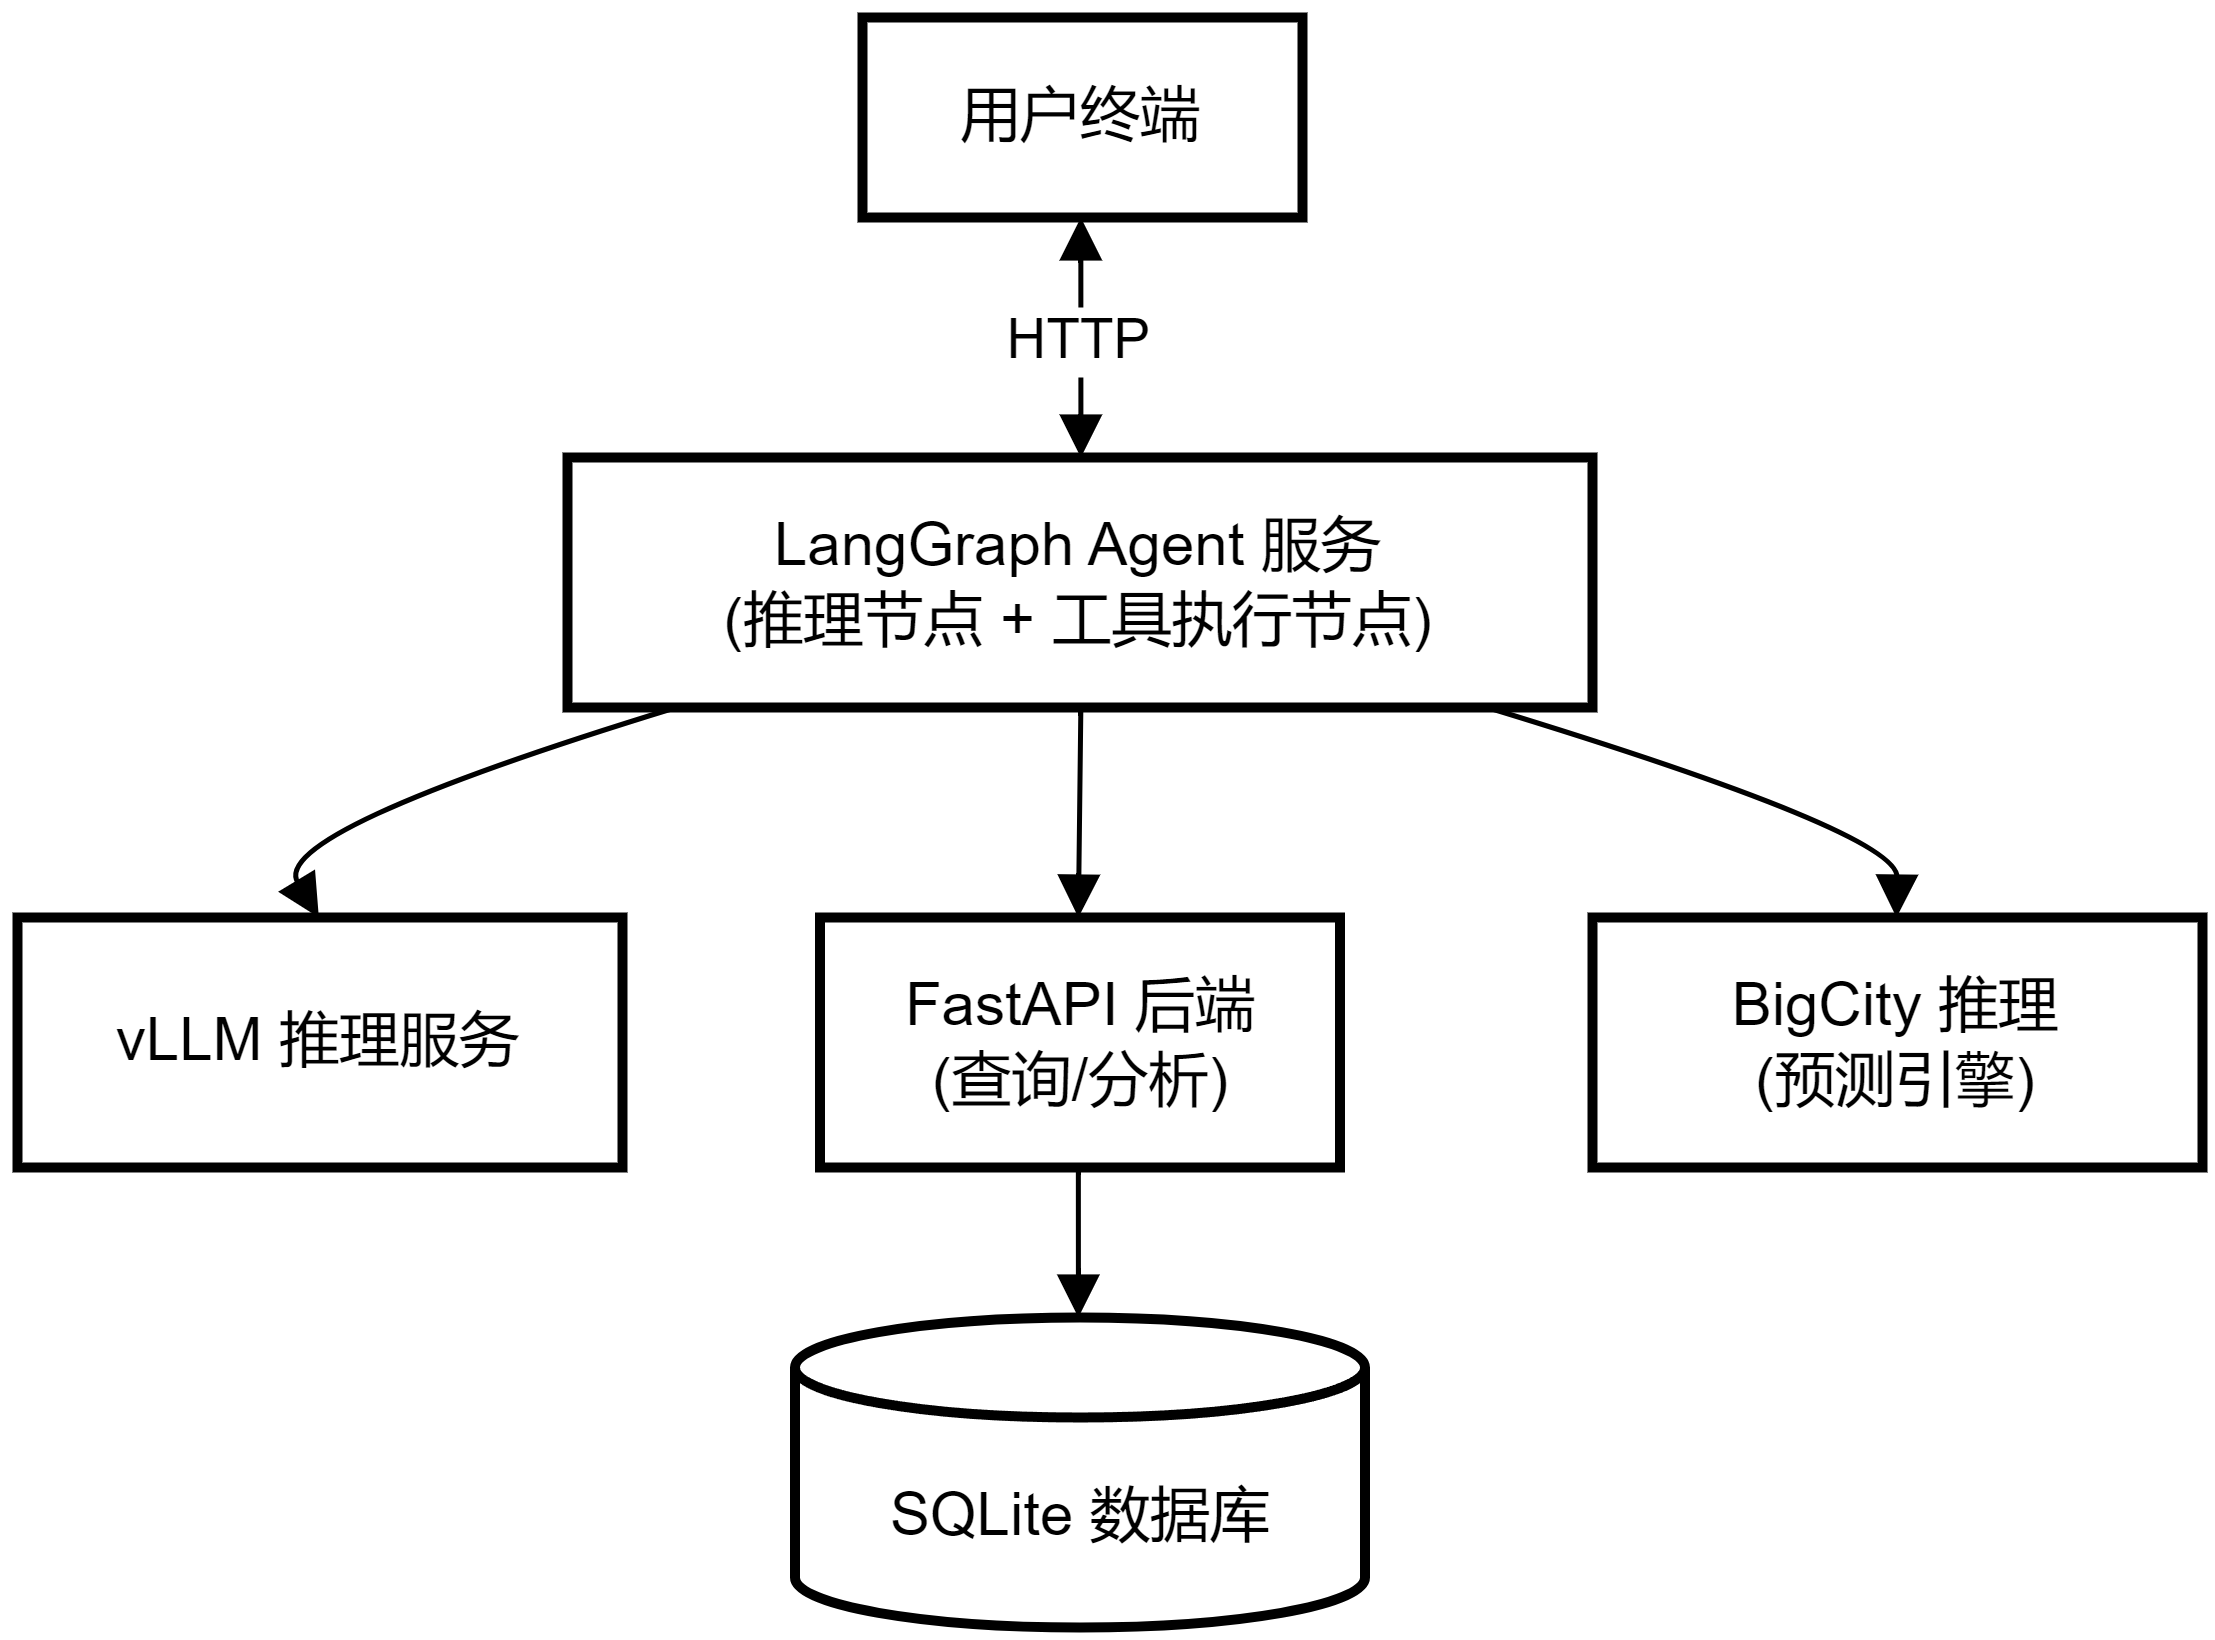
\includegraphics[width=0.85\textwidth]{figure/部署架构图.drawio.png}
  \caption{系统后端部署架构图}
  \label{fig:deployment-architecture}
\end{figure}

从后端实现架构来看，如上图所示，整个系统不是一个大一统的程序，而是由多个独立的服务组成的分布式系统，各个服务之间通过 HTTP 接口进行通信。之所以这样设计，是因为系统中的几个任务对计算资源的要求差异很大。大语言模型的推理需要 GPU 加速，交通数据的存储和查询需要磁盘 I/O，预测引擎的数值计算需要大量的 CPU 或 GPU 算力。如果把这些任务都放到同一个进程里跑，不仅资源调度会互相争抢，而且任何一个模块出问题都可能导致整个系统瘫痪。所以有必要把这些任务拆分成独立的服务，每个服务运行在自己的进程中，使用最适合它的硬件资源，通过接口调用的方式协同工作。按照职责的不同，后端架构可以分为三个层次，每一层都有清晰的划分，做到各司其职。

第一层是 Agent 调度层，也是整个系统中唯一涉及大模型推理的层次。这一层运行基于 LangGraph 的状态图逻辑，包含推理节点和工具执行节点两个核心模块。推理节点负责调用大语言模型进行意图理解和任务分解，把用户的自然语言指令拆解成具体的工具调用序列。工具执行节点负责接收这些调用指令并转发给下层服务。关键的一点是，Agent 调度层不直接处理任何数据——它不连接数据库、不运行预测模型、不进行数值计算。所有的数据查询和计算请求都封装成 HTTP 请求，转发给后端接口层去处理。这种设计把推理逻辑和数据逻辑完全分离开来，Agent 服务只需要关心“调用什么工具、传什么参数”，不需要关心“数据存在哪里、怎么查出来”。这样如果需要对 Agent 的逻辑做调整（比如修改提示词、切换底层大模型），只涉及调度层的代码变更，数据服务和接口服务的代码完全不受影响。

第二层是后端接口层，它是 Agent 调度层和数据存储层之间的桥梁。这一层基于 FastAPI 框架开发，对外暴露三个 RESTful 接口，分别对应三个工具。第一个是态势查询接口（/flow/point），接收实体 ID 和时间参数，从数据库中查找对应的记录，返回该实体在指定时刻的流量、速度和占有率等瞬时交通状态。第二个是历史趋势查询接口（/flow/history），在获取当前时刻数据的基础上，额外拉取过去一段时间的连续历史序列，返回带有时间维度的多维数据。这个接口在返回之前会做一次特征聚合——只保留流量变化明显的那些时间节点，减少传给大模型的数据量。第三个是预测计算接口（/predict），接收目标路段 ID 和预测时间跨度参数，自动遍历目标路段及其周边路段，从数据库拉取各自的历史流量序列，按时间戳对齐后组装成完整的时空特征矩阵，然后调用底层的预测推理引擎进行计算，最后从预测结果中提取目标路段的预测序列并返回。FastAPI 的异步请求处理机制使得这三个接口在同时被调用时可以并发运行，当一个请求在等待数据库 I/O 时，服务器可以切换去处理其他请求，不会阻塞整个服务。此外，后端接口层还集成了日志记录模块，每次 API 调用的时间、参数和返回值都会被记录下来，便于后续排查问题。

第三层是数据存储层，负责所有交通数据的持久化和访问。交通数据按照原子文件格式（.geo、.rel、.dyna）组织存储在 SQLite 数据库中。数据库的访问被封装在数据访问层中，后端接口层通过 数据访问层提供的接口来读写数据，不直接编写 SQL 语句。数据访问层内部使用 sqlite3.Row 工厂模式，查询结果以结构化的键值对形式返回，避免了数据在模块之间传递时出现格式不一致的问题。这种封装的好处在于，如果将来需要把 SQLite 换成 PostgreSQL 或者其他数据库，只需要修改 数据访问层的实现代码，后端接口层和 Agent 调度层的代码不需要做任何改动。BigCity 预测模型作为独立的推理引擎，单独部署在一台 GPU 服务器上，通过通信接口接收前端组装好的时空特征矩阵，运行模型推理，然后将预测结果返回。预测引擎和后端接口层之间也是松耦合的，两者通过预先定义好的接口协议通信，不共享任何内存或存储资源。这意味着如果将来有更先进的时空预测模型出现，只需要把新模型以相同的接口协议部署到 GPU 服务器上替换掉 BigCity，后端接口层和 Agent 调度层的代码完全不需要修改。

这套基于 ReAct 和 LangGraph 的智能体流程，加上原子文件、MCP 和 BigCity 时空预测模型，就构成了整个系统的完整技术路线。从数据表示到工具调用再到预测推理，每一层都有明确的分工和标准的接口：原子文件层负责将多源异构数据统一为标准格式，解决"数据怎么存"的问题；MCP 协议层将原子文件封装为标准化工具接口，解决"数据怎么调"的问题；ReAct 循环层负责智能体的意图理解和多步推理，解决"任务怎么做"的问题；BigCity 预测层负责交通状态的数值预测，解决"未来怎么推"的问题。四层各司其职，层与层之间通过标准化的接口协议通信，任意一层的内部实现发生变化都不会影响其他层的正常运行，保证了系统的可扩展性和灵活性。
